\documentclass{beamer}
\usepackage{booktabs}
\usepackage{hyperref}
\usepackage{graphicx}
\usepackage{multirow}
\usepackage{bbm}
\usepackage{amsmath}
\usepackage{algorithm}
\usepackage{algorithmic}
% \usepackage{custom_commands}
\usepackage{bm}
\usetheme{Szeged}
\usefonttheme{default}
\usecolortheme{beaver}
%Information to be included in the title page:
\title{NTK-SAP: Improving neural network pruning by aligning training dynamics}
\author[]{Yite Wang\inst{1}, Dawei Li\inst{1}, Ruoyu Sun\inst{2}\inst{3}}
\institute[]{
\inst{1}
University of Illinois Urbana-Champaign, USA \\
\inst{2}
Shenzhen International Center for Industrial and Applied Mathematics, \\ Shenzhen Research Institute of Big Data \\
\inst{3}
School of Data Science, The Chinese  University of Hong Kong, Shenzhen, China \\
}
\date{2023}

\begin{document}

\frame{\titlepage}

\section{Motivation}
\begin{frame}{Recall: Saliency score used in foresight pruning}

Foresight pruning methods prune the connections $\theta_0^j$ based on \textbf{``saliency scores''} which measures their importance.

\small 
\textbf{SNIP. \cite{snip}} $S_{\text{SNIP}}(m^j)=\left|\frac{\partial \mathcal{L}(\boldsymbol{\theta}_0 \odot \boldsymbol{m}; D)}{\partial \theta_0^j} \cdot \theta_0^j\right|$
% \textbf{SNIP.} $S_{\text{SNIP}}(m^j)=\left| \loss \cdot \theta_0^j\right|$

\textbf{GraSP. \cite{grasp}} $S_{\text{GraSP}}(m^j)=-\left[H(\boldsymbol{\theta}_0 \odot \boldsymbol{m}; D)\frac{\partial \mathcal{L}(\boldsymbol{\theta}_0  \odot \boldsymbol{m}; D)}{\partial \boldsymbol{\theta}_0}\right]^j \cdot \theta_0^j$


\textbf{Synflow. \cite{synflow}} $S_{\text{Synflow}}(m^j)=\left|\frac{\partial \sum_k f(\mathbbm{1};{|\boldsymbol{\theta}_0| \odot \boldsymbol{m}})_k}{\partial |\theta_0^j|} \cdot |\theta_0^j|\right|$

\normalsize
Most saliency scores are related to the initial few steps of training: may not be good choices for later stages of training.
\end{frame}

\begin{frame}{Motivation: Neural tangent kernel (NTK).}
\textbf{Neural Tangent Kernel (NTK)} for a network $f$ parameterized by $\theta$, and the training set $\mathcal{X}$ is
\begin{align*}
    \hat{\boldsymbol{\Theta}}(\mathcal{X},\mathcal{X}; \boldsymbol{\theta}) \triangleq \nabla_{\boldsymbol{\theta}}f(\mathcal{X};\boldsymbol{\theta}) \nabla_{\boldsymbol{\theta}}f(\mathcal{X};\boldsymbol{\theta})^T.
\end{align*}

\end{frame}
\begin{frame}{Motivation: NTK eigenspectrum.}
\textbf{The condition number of the NTK is related to neural network optimization.} 
% The condition number of the NTK is known to be important in neural network optimization. \\~\
% For large-width networks, the mean prediction of the neural network in the eigenbasis with the smallest magnitude of NTK, the convergence rate is related to the condition number of the NTK. 

% The condition number of the NTK is important in NN optimization.
For large-width networks, the convergence rate is related to the condition number of the NTK.

\end{frame}

\begin{frame}{Motivation: NTK eigenspectrum.}
    \textbf{The entire spectrum of the NTK is a better measure.} 
    % However, the smallest and the largest eigenvalues only provide very limited information on the optimization property of the DNNs. Compared to only considering the condition number of the NTK, controlling the entire eigenspectrum may be a better way to ensure the satisfactory optimization performance of DNNs.
    Condition number provides very limited information on the optimization property of the DNNs. Entire eigenspectrum may be a better measure to control different eigenmodes.
\end{frame}

\section{Our Approach}

\begin{frame}{NTK-SAP: Using NTK nuclear norm as a scalar indicator}
    Advantages of using the nuclear norm of NTK: \\
    \begin{enumerate}
        \item \textbf{Computational efficiency.} 
        \begin{itemize}
            \item The computational cost of computing all the eigenvalues is expensive.
            \item But, trace norm can be efficiently approximated.
        \end{itemize} 
        % The computational cost of computing all the eigenvalues would be too expensive. On the contrary, trace norm can be efficiently approximated.
        \item \textbf{Implicitly preserve the entire spectrum.}  \\~\
        Removing weights with a smaller saliency score is less likely to induce significant change to the eigenvalue distribution.
        % The saliency score for each weight measures the change of the metric (here it is the trace norm of the NTK) when removing the weight. More precisely, removing weights with a smaller saliency score is less likely to induce significant change to the eigenvalue distribution.
    \end{enumerate}
    

    
\end{frame}



\begin{frame}{NTK-SAP: Approximating nuclear norm of analytic NTK}
    \textbf{Nuclear norm as a proxy of the whole spectrum.} 
\begin{align*}
\|\boldsymbol{\Theta}_0\|_{*}=\|\boldsymbol{\Theta}_0\|_\text{tr}=\|\nabla_{\boldsymbol{\theta}_0}f(\mathcal{X};\boldsymbol{\theta}_0)\|_{F}^2.
\end{align*}
\textbf{Finite difference approximation.} We use the finite difference expression to approximate the Jacobian norm. 
\begin{align*}
    \frac{1}{\epsilon}\mathbb{E}_{\Delta \boldsymbol{\theta} \sim \mathcal{N}(\textbf{0},\epsilon\textbf{I})}\left[\|f(\mathcal{X};\boldsymbol{\theta}_0)-f(\mathcal{X};\boldsymbol{\theta}_0+\Delta\boldsymbol{\theta})\|_2^2\right]
\end{align*}

\end{frame}

\begin{frame}{NTK-SAP: Fixed-weight-NTK and analytic NTK}
    \textbf{Fixed-weight-NTK:} NTK defined for the given (finite-width) architecture with a random configuration (initialization).
    
    \textbf{Analytic NTK \cite{jacot2018ntk}:}  The asymptotic limit of the fixed-weight-NTK as the network width goes to infinity. The analytic NTK is the one studied in NTK theory.
    
    \begin{alertblock}{Our Conjecture}
    We think the spectrum of the analytic NTK may serve as a performance indicator of a certain architecture throughout the whole training process. \\~\
    
    \alert{Hence, we need to approximate the analytic NTK with the fix-weight-NTK.}
    \end{alertblock}
     
\end{frame}

\begin{frame}{NTK-SAP: Multi-sampling fixed-weight-NTK}
% While a single fixed-weight-NTK can be viewed as an approximation
% of the analytic NTK,  the expectation of fixed-weight-NTKs (expecation over random draw of weight configurations) shall be a better approximation. 

\begin{alertblock}{Approximate analytic NTK with the fixed-weight-NTK}
    The expectation of fixed-weight-NTKs (expecation over random draw of weight configurations) shall be a better approximation compared to a single fixed-weight-NTK. 
\end{alertblock}


Specifically, with $R$ random weight configurations $\boldsymbol{\theta}_{0,r} \overset{\mathrm{iid}}{\sim} \mathcal{P}$, $\Delta \boldsymbol{\theta}_{i} \overset{\mathrm{iid}}{\sim} \mathcal{N}(\textbf{0},\epsilon\textbf{I})$, we use the following stabilized version of the saliency score: 
% \tiny
\begin{align*}
    \left|\frac{\partial \frac{1}{R} \sum_{r=1}^R \left[\|f(\mathcal{X};\boldsymbol{\theta}_{0,r}\odot \textbf{m})-f(\mathcal{X};(\boldsymbol{\theta}_{0,r}+\Delta\boldsymbol{\theta}_i)\odot \textbf{m})\|_2^2\right]}{\partial m^j}\right|. 
\end{align*} 

\end{frame}

% \begin{frame}{NTK-SAP}
% \textbf{Approximating the training set with Gaussian noise.} We use the inputs of the pruning dataset $\mathbf{X}_D$ to approximate the whole training inputs $\mathcal{X}$. 
% \begin{align*}
% \left|\frac{\partial \mathbb{E}_{\Delta \boldsymbol{\theta} \sim \mathcal{N}(\textbf{0},\epsilon\textbf{I})}\left[\|f(\mathbf{X}_D;\boldsymbol{\theta}_0\odot {m})-f(\mathbf{X}_D;(\boldsymbol{\theta}_0+\Delta\boldsymbol{\theta})\odot m)\|_2^2\right]}{\partial m^j}\right|
% \end{align*}
% \end{frame}

\begin{frame}{NTK-SAP: Data-agnostic}
\textbf{Replacing training set with random Gaussian noise.} \\~\
Furthermore, we find that using standard Gaussian noise $\mathcal{Z}\sim \mathcal{N}(\textbf{0},\textbf{I})$ can work well, which makes NTK-SAP purely data-agnostic. \\
We have the final data-agnostic NTK-SAP with its saliency score:
\begin{align*}
     \left|\frac{\partial \frac{1}{|D|} \sum_{i=1}^{|D|} \left[\|f(\mathbf{z}_{i};\boldsymbol{\theta}_{0,i}\odot \textbf{m})-f(\mathbf{z}_{i};(\boldsymbol{\theta}_{0,i}+\Delta\boldsymbol{\theta}_{i})\odot \textbf{m})\|_2^2\right]}{\partial m^j}\right| \label{eq:multi-init-final}
\end{align*}     
\end{frame}

\begin{frame}{NTK-SAP}
\begin{algorithm}[H]
\caption{Neural Tagent Kernel Spectrum-Aware Pruning (NTK-SAP)}
% \caption{Our algorithm}
% \label{alg:ntksap}
\begin{algorithmic}[1]
{\tiny
\REQUIRE Dense network $f(\cdot; \boldsymbol{\theta} \odot \mathbf{m})$, final density $d$, iteration steps $T$, batch size of noise input $B$, perturbation hyperparameter $\epsilon$
\STATE Initialize $\mathbf{m}=\mathbbm{1}$
\FOR{$t$ in $\left[1, \cdots, T\right]$}
  \FOR{$i$ in $\left[1, \cdots, B\right]$} 
    \STATE Reinitialize neural network with $\boldsymbol{\theta}_{0,i} \overset{\mathrm{iid}}{\sim} \mathcal{P}$
    \STATE Sample noise input $\mathbf{z}_{i} \overset{\mathrm{iid}}{\sim} \mathcal{N}(\textbf{0},\textbf{I})$ and parameter perturbation $\Delta \boldsymbol{\theta}_{i} \overset{\mathrm{iid}}{\sim} \mathcal{N}(\textbf{0},\epsilon\textbf{I})$
    % \STATE Evaluate saliency scores $\left[\mathcal{S}(\mathbf{m})\right]_i$ based on Equation (\ref{eq:multi-init-final})
    \STATE Evaluate saliency scores $\left[\mathcal{S}(\mathbf{m})\right]_i$
 \ENDFOR
 \STATE Calculate $\mathcal{S}(\mathbf{m})=\left|\sum_{i=1}^B\left[\mathcal{S}(\mathbf{m})\right]_i\right|$ 
 \STATE Compute $(1-d^{\frac{t}{T}})$ percentile of $\mathcal{S}(\mathbf{m})$ as threshold $\tau$
 \STATE Update mask $\mathbf{m} \leftarrow \mathbf{m} \odot (\mathcal{S}(\mathbf{m})>\tau) $
\ENDFOR
\RETURN Final mask $\mathbf{m}$
}
\end{algorithmic}
\end{algorithm}
\end{frame}

\section{Results}
\begin{frame}{Experiment results}
    \begin{figure}
  \centering
    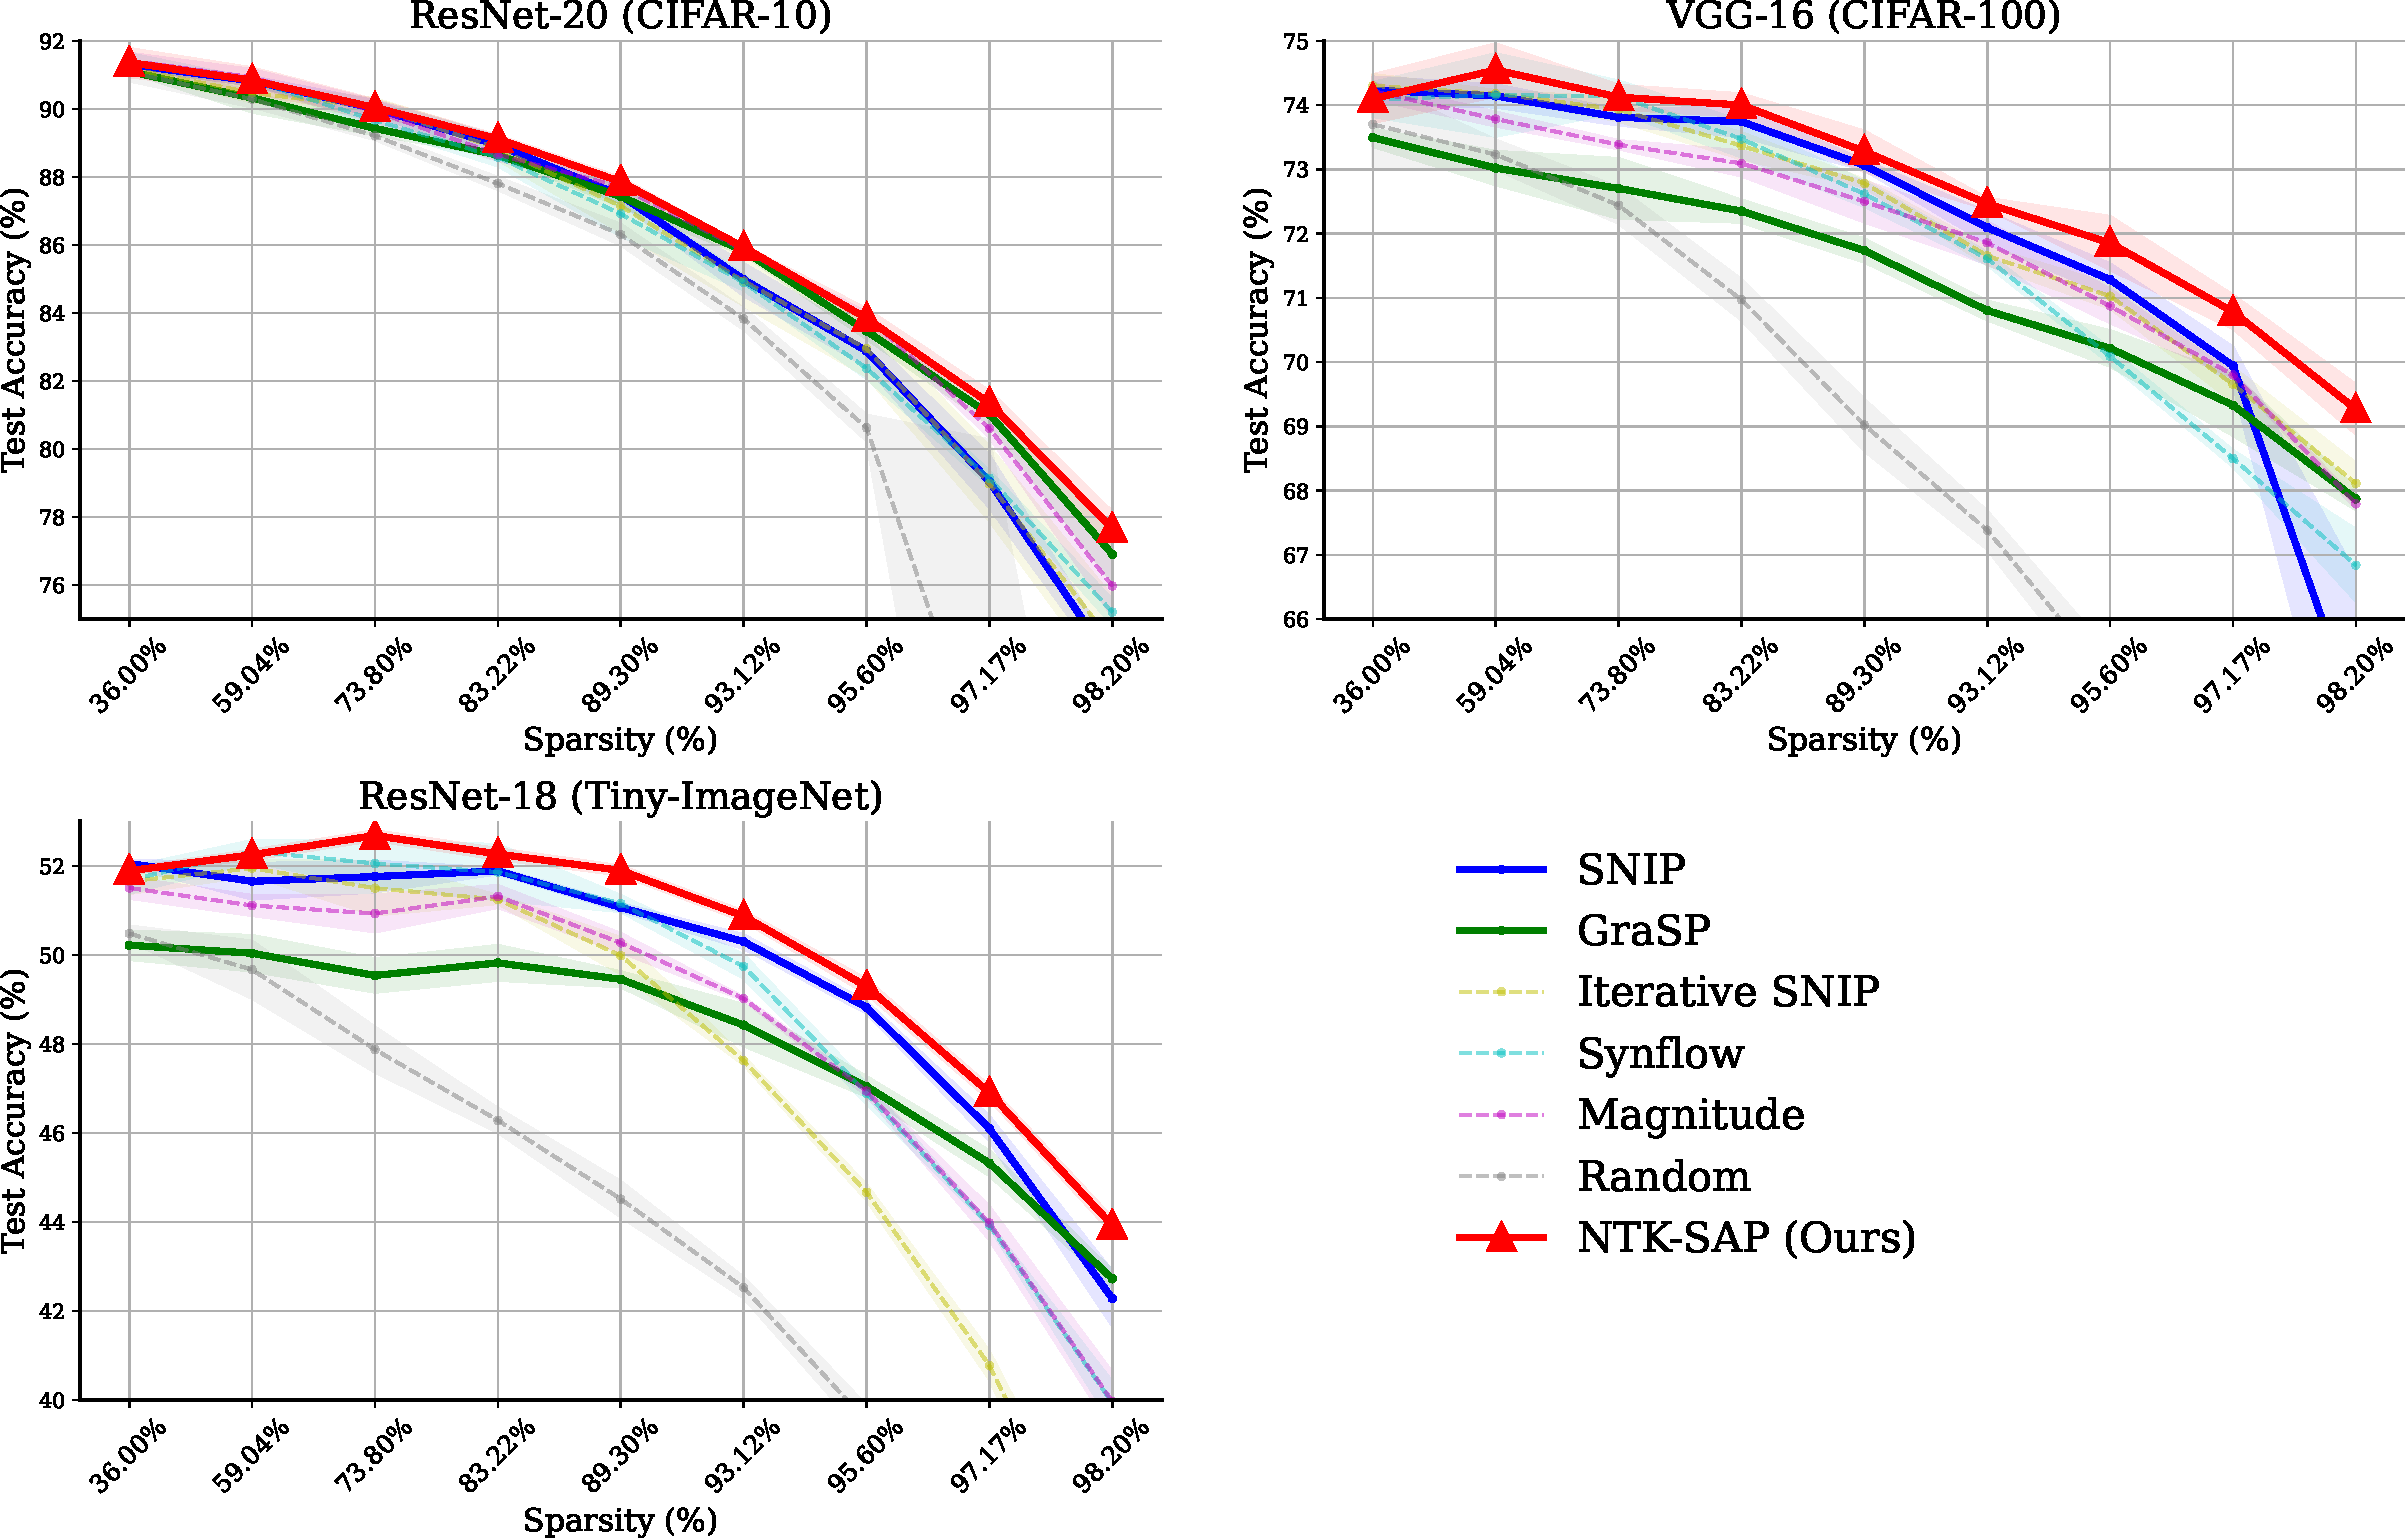
\includegraphics[width=0.75\textwidth]{iclr2023/plots/test_single_914_main.pdf}
   \caption{Performance of NTK-SAP against other foresight pruning methods. Results are averaged over 3 random seeds, and the shaded areas denote the standard deviation.}
   % \label{fig:main-comparison}
%   \vspace{-0.5cm}
\end{figure}
\end{frame}


\begin{frame}{Results on ImageNet}
    \begin{table}
        \centering
        \caption{
        Test performance of foresight pruning methods on the ImageNet dataset. Best results are in \textbf{bold}; second-best results are \underline{underlined}.}
        \resizebox{0.75\textwidth}{!}{
        \begin{tabular}[b]{ l cccccc}
        \\
        \hline
        \toprule
        Network & \multicolumn{2}{c}{\textbf{ResNet-18}} &\multicolumn{2}{c}{\textbf{ResNet-50}} \\
        \midrule
        Sparsity percentage & 89.26\% & 95.60\% &  89.26\% & 95.60\% \\ 
        \midrule
        (Dense Baseline) &69.98&&76.20& \\
        \midrule
        Synflow &57.30&45.65& 66.81 & 58.88 \\
        SNIP &57.41 &45.04& 60.98 & 40.69 \\
        Iterative SNIP &52.97 &37.44& 52.53 & 36.82 \\
        GraSP &58.16&\underline{49.17}& \underline{67.74}& \underline{59.73}\\
        Magnitude &\underline{58.75}&48.50&66.80&43.79 \\
        Random &54.48&42.80&65.30&56.53 \\
        \midrule
        \midrule
        \textbf{NTK-SAP (Ours)} &\textbf{58.87}&\textbf{49.43}&\textbf{68.28}&\textbf{60.79} \\
        
        \bottomrule
        \end{tabular}
        }
    \end{table}
\end{frame}

\begin{frame}{Results}
    \begin{center}
        \Huge Thank you!
    \end{center}
    
\end{frame}

\begin{frame}
\tiny
\frametitle{bibliography}
\bibliographystyle{amsalpha}
\bibliography{iclr2023/iclr2023_conference}
\end{frame}

\end{document}